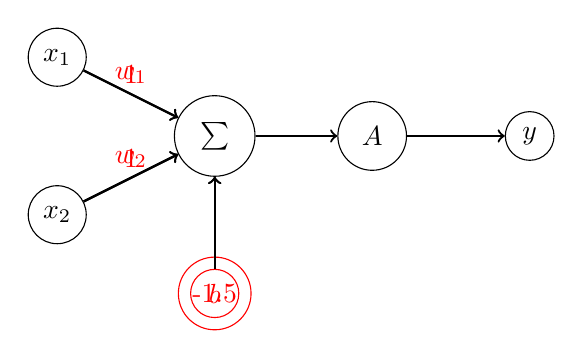
\begin{tikzpicture}[xscale = 2, yscale = 2]
  \node[draw, circle] (X1) at (0, 0){
    $x_{1}$
  };

  \node[draw, circle] (X2) at (0, -1){
    $x_{2}$
  };

  \uncover<1>{
    \node[draw, circle, red] (bias) at (1, -1.5){
      $b$
    };
  }

  \uncover<2->{
    \node[draw, circle, red] (biasVal) at (1, -1.5){
      -1.5
    };
  }

  \node[draw, circle] (sum) at (1, -0.5){
    \scalebox{1}{
      $\sum$
    }
  };

  \node[draw, circle] (activation) at (2, -0.5){
    \scalebox{1}{
      $A$
    }
  };

  \node[draw, circle] (y) at (3, -0.5){
    $y$
  };

  \uncover<1>{
    \draw[thick, ->] (X1) -- node [above, red]{$w_{1}$} (sum);
    \draw[thick, ->] (X2) -- node [above, red]{$w_{2}$} (sum);
    \draw[thick, ->] (bias) -- (sum);
  }

  \uncover<2->{
    \draw[thick, ->] (biasVal) -- (sum);
    \draw[thick, ->] (X1) -- node [above, red]{1} (sum);
    \draw[thick, ->] (X2) -- node [above, red]{1} (sum);
  }

  \draw[thick, ->] (sum) -- (activation);
  \draw[thick, ->] (activation) -- (y);
\end{tikzpicture}
